\documentclass[aspectratio=169, 11pt]{beamer}

\usetheme{Madrid}
\usecolortheme{default}

\definecolor{msNavy}{HTML}{1B2A4A}
\definecolor{msTeal}{HTML}{0891B2}
\definecolor{msAccent}{HTML}{06B6D4}
\definecolor{msLight}{HTML}{E0F2FE}
\definecolor{msGray}{HTML}{64748B}
\definecolor{msRed}{HTML}{DC2626}
\definecolor{msGreen}{HTML}{16A34A}
\definecolor{msOrange}{HTML}{EA580C}
\definecolor{msBg}{HTML}{F8FAFC}

\setbeamercolor{palette primary}{bg=msNavy, fg=white}
\setbeamercolor{palette secondary}{bg=msTeal, fg=white}
\setbeamercolor{palette tertiary}{bg=msNavy, fg=white}
\setbeamercolor{structure}{fg=msNavy}
\setbeamercolor{title}{fg=white, bg=msNavy}
\setbeamercolor{frametitle}{fg=white, bg=msNavy}
\setbeamercolor{block title}{bg=msTeal, fg=white}
\setbeamercolor{block body}{bg=msLight, fg=msNavy}
\setbeamercolor{block title alerted}{bg=msRed, fg=white}
\setbeamercolor{block body alerted}{bg=msLight, fg=msNavy}
\setbeamercolor{block title example}{bg=msGreen, fg=white}
\setbeamercolor{block body example}{bg=msLight, fg=msNavy}
\setbeamercolor{itemize item}{fg=msTeal}
\setbeamercolor{itemize subitem}{fg=msAccent}
\setbeamercolor{footline}{fg=msGray}
\setbeamercolor{normal text}{fg=msNavy}

\setbeamerfont{title}{size=\Large, series=\bfseries}
\setbeamerfont{frametitle}{size=\large, series=\bfseries}
\setbeamerfont{framesubtitle}{size=\small, series=\normalfont}
\setbeamertemplate{navigation symbols}{}

\setbeamertemplate{footline}{
  \leavevmode%
  \hbox{%
    \begin{beamercolorbox}[wd=.33\paperwidth,ht=2.5ex,dp=1ex,left]{footline}%
      \hspace*{2ex}\textcolor{msGray}{\footnotesize MediSpark | 23AID302}
    \end{beamercolorbox}%
    \begin{beamercolorbox}[wd=.34\paperwidth,ht=2.5ex,dp=1ex,center]{footline}%
      \textcolor{msGray}{\footnotesize Team B11 -- 0\textsuperscript{th} Review}
    \end{beamercolorbox}%
    \begin{beamercolorbox}[wd=.33\paperwidth,ht=2.5ex,dp=1ex,right]{footline}%
      \textcolor{msGray}{\footnotesize \insertframenumber/\inserttotalframenumber}\hspace*{2ex}
    \end{beamercolorbox}}%
  \vskip0pt%
}

\usepackage[utf8]{inputenc}
\usepackage[T1]{fontenc}
\usepackage{lmodern}
\usepackage{graphicx}
\usepackage{booktabs}
\usepackage{array}
\usepackage{colortbl}
\usepackage{tikz}
\usepackage{pifont}
\usepackage{hyperref}
\usepackage{multicol}
\usepackage{ragged2e}

\usetikzlibrary{shapes.geometric, arrows.meta, positioning, calc}

\newcolumntype{L}[1]{>{\raggedright\arraybackslash}p{#1}}
\newcolumntype{C}[1]{>{\centering\arraybackslash}p{#1}}

\title[MediSpark]{\textbf{MediSpark}}
\subtitle{A Scalable Multi-Disease Clinical Risk Prediction Engine}
\author[Team B11]{
  Suman Maitreya \textnormal{\small (CB.AI.U4AID24156)} \and
  Rajkumar R \textnormal{\small (CB.AI.U4AID24143)} \and
  Harish K \textnormal{\small (CB.AI.U4AID24118)} \and
  GRS Kartheek \textnormal{\small (CB.AI.U4AID24116)}
}
\institute[Amrita]{
  23AID302 -- Big Data Analytics \\
  Supervisor: Dr.\ Sreeja B P \\[4pt]
  \textit{Amrita Vishwa Vidyapeetham, Coimbatore}
}
\date{0\textsuperscript{th} Review -- July 2026}

\begin{document}

% ---- SLIDE 1: TITLE ----
{
\setbeamertemplate{footline}{}
\begin{frame}[plain]
\begin{tikzpicture}[remember picture, overlay]
  \fill[msNavy] (current page.north west) rectangle (current page.south east);
  \fill[msTeal] ([yshift=-3.2cm]current page.north west) rectangle ([yshift=-3.25cm]current page.north east);
  \fill[msBg] ([yshift=-5.5cm]current page.north west) rectangle (current page.south east);
  \fill[msTeal, opacity=0.15] ([xshift=11cm, yshift=-2cm]current page.north west) circle (2.5cm);
  \fill[msAccent, opacity=0.1] ([xshift=13cm, yshift=-4cm]current page.north west) circle (1.8cm);
\end{tikzpicture}

\vspace{0.3cm}
\begin{center}
  {\footnotesize\textcolor{msAccent}{23AID302 -- BIG DATA ANALYTICS \textbar\ 0\textsuperscript{TH} REVIEW \textbar\ TEAM B11}}\\[0.6cm]
  {\Huge\textbf{\textcolor{white}{MediSpark}}}\\[0.3cm]
  {\normalsize\textcolor{gray!70}{A Scalable Multi-Disease Clinical Risk Prediction Engine}}\\[0.15cm]
  {\scriptsize\textcolor{msAccent}{Apache Spark $\cdot$ Hadoop HDFS $\cdot$ Scala $\cdot$ Spark MLlib $\cdot$ Docker}}
\end{center}

\vspace{1.0cm}
\begin{center}
  \begin{minipage}{0.8\textwidth}
    \centering
    {\small\textcolor{msNavy}{
      \textbf{Suman Maitreya} \textbar\ CB.AI.U4AID24156 \quad
      \textbf{Rajkumar R} \textbar\ CB.AI.U4AID24143 \\[4pt]
      \textbf{Harish K} \textbar\ CB.AI.U4AID24118 \quad
      \textbf{GRS Kartheek} \textbar\ CB.AI.U4AID24116 \\[8pt]
      \textcolor{msGray}{23AID302 -- Big Data Analytics \quad $\cdot$ \quad Supervisor: Dr.\ Sreeja B P} \\
      \textcolor{msGray}{Amrita Vishwa Vidyapeetham, Coimbatore}
    }}
  \end{minipage}
\end{center}
\end{frame}
}

% ---- SLIDE 2: INTRODUCTION ----
\begin{frame}{Introduction to the Problem Domain}
\framesubtitle{Healthcare Meets Big Data}

\begin{columns}[T]
\begin{column}{0.62\textwidth}
  \begin{itemize}
    \item The healthcare sector generates \textbf{millions of patient records daily} from hospitals, wearables, labs, and electronic health records (EHRs).
    \vspace{0.2cm}
    \item Traditional systems \textbf{cannot process} this volume, velocity, and variety of data in real time.
    \vspace{0.2cm}
    \item Chronic diseases --- heart disease, diabetes, stroke, and lung cancer --- cause \textbf{over 70\% of global deaths} annually.
    \vspace{0.2cm}
    \item Early detection through \textbf{data-driven prediction} can save millions of lives.
    \vspace{0.2cm}
    \item Big Data technologies like \textbf{Apache Spark} and \textbf{Hadoop HDFS} now enable scalable, real-time healthcare analytics.
  \end{itemize}
\end{column}

\begin{column}{0.35\textwidth}
  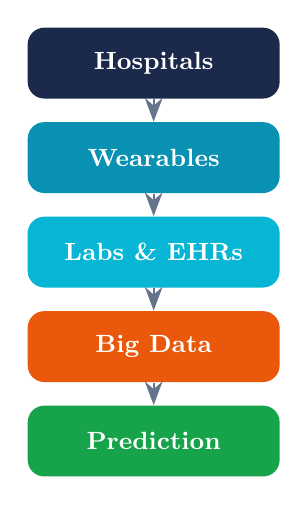
\begin{tikzpicture}[
    box/.style={rounded corners=6pt, minimum width=3.2cm, minimum height=0.9cm, align=center, font=\small\bfseries, text=white},
  ]
    \node[box, fill=msNavy] (h) at (0, 4.0) {Hospitals};
    \node[box, fill=msTeal] (w) at (0, 2.8) {Wearables};
    \node[box, fill=msAccent] (l) at (0, 1.6) {Labs \& EHRs};
    \node[box, fill=msOrange] (d) at (0, 0.4) {Big Data};
    \node[box, fill=msGreen] (p) at (0, -0.8) {Prediction};

    \draw[-{Stealth[length=3mm]}, thick, msGray] (h.south) -- (w.north);
    \draw[-{Stealth[length=3mm]}, thick, msGray] (w.south) -- (l.north);
    \draw[-{Stealth[length=3mm]}, thick, msGray] (l.south) -- (d.north);
    \draw[-{Stealth[length=3mm]}, thick, msGray] (d.south) -- (p.north);
  \end{tikzpicture}
\end{column}
\end{columns}
\end{frame}

% ---- SLIDE 3: 5 V's ----
\begin{frame}{Importance of the Domain}
\framesubtitle{Why Healthcare Big Data Matters}

\vspace{0.3cm}
\begin{center}
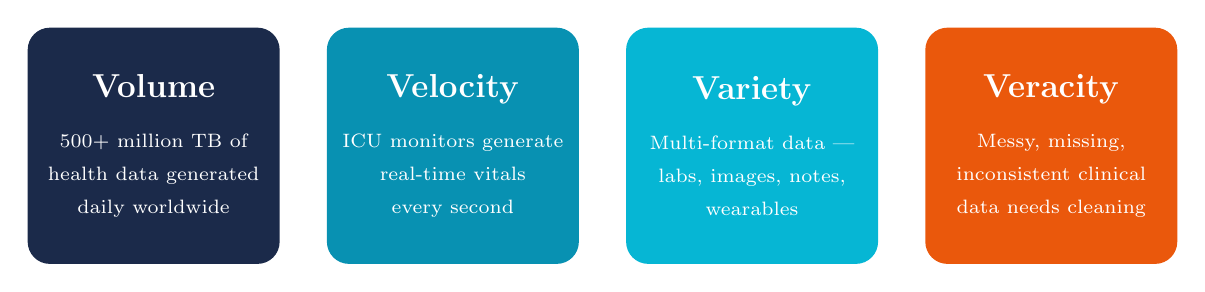
\begin{tikzpicture}[
  card/.style={rounded corners=8pt, minimum width=3.2cm, minimum height=3.0cm, align=center, text=white},
]
  \node[card, fill=msNavy] (v1) at (0, 0) {
    {\large\textbf{Volume}}\\[6pt]
    {\scriptsize 500+ million TB of}\\
    {\scriptsize health data generated}\\
    {\scriptsize daily worldwide}
  };
  \node[card, fill=msTeal] (v2) at (3.8, 0) {
    {\large\textbf{Velocity}}\\[6pt]
    {\scriptsize ICU monitors generate}\\
    {\scriptsize real-time vitals}\\
    {\scriptsize every second}
  };
  \node[card, fill=msAccent] (v3) at (7.6, 0) {
    {\large\textbf{Variety}}\\[6pt]
    {\scriptsize Multi-format data ---}\\
    {\scriptsize labs, images, notes,}\\
    {\scriptsize wearables}
  };
  \node[card, fill=msOrange] (v4) at (11.4, 0) {
    {\large\textbf{Veracity}}\\[6pt]
    {\scriptsize Messy, missing,}\\
    {\scriptsize inconsistent clinical}\\
    {\scriptsize data needs cleaning}
  };
\end{tikzpicture}
\end{center}

\vspace{0.4cm}
\begin{center}
  \colorbox{msLight}{\parbox{0.85\textwidth}{\centering\small
    \textcolor{msNavy}{\textbf{Value:} Predictive analytics can reduce misdiagnosis by 30\% and enable early intervention for chronic diseases.}
  }}
\end{center}

\vspace{0.2cm}
{\tiny\textcolor{msGray}{\hfill Source: WHO Global Health Observatory \& IDC Data Age 2025 Report}}

\end{frame}

% ---- SLIDE 4: PROBLEM STATEMENT ----
\begin{frame}{Problem Statement}

\vspace{0.5cm}
\begin{center}
  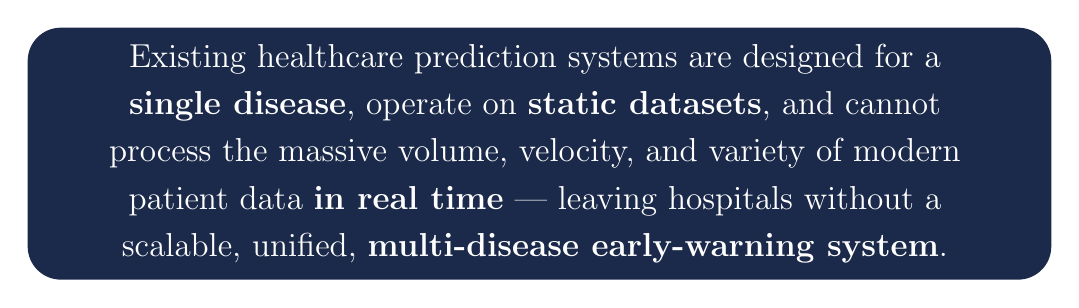
\begin{tikzpicture}
    \node[rounded corners=12pt, fill=msNavy, text=white, minimum width=13cm, minimum height=3.2cm, align=center] {
      \parbox{11.5cm}{\centering\large
        Existing healthcare prediction systems are designed for a\\[3pt]
        \textbf{single disease}, operate on \textbf{static datasets}, and cannot\\[3pt]
        process the massive volume, velocity, and variety of modern\\[3pt]
        patient data \textbf{in real time} --- leaving hospitals without a\\[3pt]
        scalable, unified, \textbf{multi-disease early-warning system}.
      }
    };
  \end{tikzpicture}
\end{center}

\vspace{0.5cm}

\begin{columns}[T]
  \begin{column}{0.32\textwidth}
    \begin{alertblock}{\ding{56}\ \ Gap 1}
      Single-disease models --- no unified multi-disease prediction exists.
    \end{alertblock}
  \end{column}
  \begin{column}{0.32\textwidth}
    \begin{alertblock}{\ding{56}\ \ Gap 2}
      Batch-only systems --- cannot score new patient records in real time.
    \end{alertblock}
  \end{column}
  \begin{column}{0.32\textwidth}
    \begin{alertblock}{\ding{56}\ \ Gap 3}
      No veracity handling --- messy, missing, inconsistent clinical data ignored.
    \end{alertblock}
  \end{column}
\end{columns}

\end{frame}

% ---- SLIDE 5: LITERATURE REVIEW ----
\begin{frame}{Literature Review --- Related Work}
\framesubtitle{Summary of Recent Research (2024--2025)}

\vspace{0.1cm}
{\small

\begin{block}{\small Paper 1: Rajendra Kumar et al.\ (2024) --- \textit{Biomedical Signal Processing \& Control}, Elsevier}
\end{block}
\vspace{-0.15cm}
\textbf{Method:} Spark-based FCM clustering + Deep Belief Network feature fusion, classified via hybrid SqueezeNet-LinkNet model for heart disease prediction.\\
\textcolor{msRed}{\textbf{Gaps:}} Single-disease $\cdot$ Batch-only $\cdot$ No HDFS $\cdot$ Complex black-box deep learning model.

\vspace{0.25cm}

\begin{block}{\small Paper 2: Fancy et al.\ (2025) --- \textit{Expert Systems}, Wiley}
\end{block}
\vspace{-0.15cm}
\textbf{Method:} Hadoop MapReduce with MRFO-based feature selection and RVM classifier tuned via Arithmetic Optimization Algorithm for healthcare big data.\\
\textcolor{msRed}{\textbf{Gaps:}} MapReduce (not Spark) $\cdot$ Single-disease $\cdot$ No streaming $\cdot$ No data-quality pipeline.

\vspace{0.25cm}

\begin{block}{\small Paper 3: Chunduru et al.\ (2024) --- \textit{SN Computer Science}, Springer}
\end{block}
\vspace{-0.15cm}
\textbf{Method:} Flask web app with CNN + Random Forest as 7 isolated single-disease models (diabetes, heart, kidney, liver, cancer, malaria, pneumonia).\\
\textcolor{msRed}{\textbf{Gaps:}} No distributed computing $\cdot$ Isolated models $\cdot$ No real-time streaming $\cdot$ Small-scale data.

}
\end{frame}

% ---- SLIDE 6: RESEARCH GAP SUMMARY ----
\begin{frame}{Research Gap}
\framesubtitle{What Existing Systems Lack vs.\ What MediSpark Provides}

\vspace{0.2cm}
\begin{center}
\renewcommand{\arraystretch}{1.35}
\begin{tabular}{@{} >{\columncolor{white}}L{6.5cm} >{\columncolor{white}}L{6.5cm} @{}}
\toprule
\rowcolor{msNavy}
\textcolor{white}{\textbf{What Exists}} & \textcolor{white}{\textbf{What MediSpark Provides}} \\
\midrule
\textcolor{msRed}{\ding{56}} \ Single-disease prediction models only &
\textcolor{msGreen}{\ding{52}} \ 4 diseases predicted simultaneously \\

\textcolor{msRed}{\ding{56}} \ No distributed HDFS-based storage &
\textcolor{msGreen}{\ding{52}} \ Full HDFS storage with 3$\times$ replication \\

\textcolor{msRed}{\ding{56}} \ No dedicated data veracity pipeline &
\textcolor{msGreen}{\ding{52}} \ IQR outlier removal, null handling, dedup \\

\textcolor{msRed}{\ding{56}} \ Streaming OR batch --- never both &
\textcolor{msGreen}{\ding{52}} \ Batch training + real-time Structured Streaming \\

\textcolor{msRed}{\ding{56}} \ Complex infra (Kafka, Cassandra) &
\textcolor{msGreen}{\ding{52}} \ Simple Docker Compose --- fully reproducible \\

\textcolor{msRed}{\ding{56}} \ No Scala-based ML Pipeline API &
\textcolor{msGreen}{\ding{52}} \ Scala Spark ML Pipeline --- production-grade \\
\bottomrule
\end{tabular}
\end{center}

\vspace{0.3cm}
\begin{center}
  \colorbox{msLight}{\parbox{0.9\textwidth}{\centering\small
    \textcolor{msNavy}{\textit{None of the reviewed works combine a unified multi-disease pipeline, HDFS-replicated storage, real-time streaming, and an auditable data-quality stage in one system.}}
  }}
\end{center}

\end{frame}

% ---- SLIDE 7: PROPOSED SYSTEM ----
\begin{frame}{Proposed System --- MediSpark Architecture}
\framesubtitle{End-to-End Distributed Clinical Risk Prediction Engine}

\vspace{0.2cm}
\begin{center}

\begin{tikzpicture}[
  stage/.style={rounded corners=6pt, minimum width=2.0cm, minimum height=1.4cm, align=center, font=\scriptsize\bfseries, text=white},
  arr/.style={-{Stealth[length=2.5mm]}, thick, msGray},
  node distance=0.4cm
]
  \node[stage, fill=msNavy]   (s1) at (0,0)    {Raw Datasets\\(Kaggle/UCI)};
  \node[stage, fill=msTeal]   (s2) at (2.7,0)  {HDFS Storage\\(3 DataNodes)};
  \node[stage, fill=msAccent] (s3) at (5.4,0)  {Data Cleaning\\(Spark/Scala)};
  \node[stage, fill=msOrange] (s4) at (8.1,0)  {Feature\\Engineering};
  \node[stage, fill=msRed]    (s5) at (10.8,0) {ML Training\\(Random Forest)};
  \node[stage, fill=msGreen]  (s6) at (13.5,0) {Real-Time\\Streaming};

  \draw[arr] (s1) -- (s2);
  \draw[arr] (s2) -- (s3);
  \draw[arr] (s3) -- (s4);
  \draw[arr] (s4) -- (s5);
  \draw[arr] (s5) -- (s6);
\end{tikzpicture}
\end{center}

\vspace{0.3cm}
\begin{columns}[T]
  \begin{column}{0.48\textwidth}
    \begin{exampleblock}{\ding{52}\ \ How It Improves}
      \begin{itemize}\small
        \item Processes \textbf{4 diseases} --- Heart, Diabetes, Stroke, Lung Cancer --- in one unified pipeline
        \item Scores new patients \textbf{every 5 seconds} via Spark Structured Streaming
        \item HDFS with \textbf{3$\times$ replication} for fault tolerance
      \end{itemize}
    \end{exampleblock}
  \end{column}
  \begin{column}{0.48\textwidth}
    \begin{exampleblock}{\ding{72}\ \ What is New (Novelty)}
      \begin{itemize}\small
        \item \textbf{Multi-disease parallelism} in a single Spark pipeline
        \item \textbf{Veracity-first} data quality stage with auditable reports
        \item \textbf{Native Scala} on JVM --- zero Python serialization overhead
        \item \textbf{Docker-based} reproducible cluster setup
      \end{itemize}
    \end{exampleblock}
  \end{column}
\end{columns}

\vspace{0.15cm}
\begin{center}
  {\small\textbf{Output:} \texttt{Patient ID \textbar\ Disease \textbar\ Risk Level (High/Medium/Low) \textbar\ Confidence \%}}
\end{center}

\end{frame}

% ---- SLIDE 8: OBJECTIVES ----
\begin{frame}{Objectives of the Project}

\vspace{0.3cm}
\begin{enumerate}
  \setlength{\itemsep}{0.35cm}

  \item[\textcolor{msTeal}{\textbf{O1}}]
    \textbf{To design} a distributed data storage and ingestion pipeline using Hadoop HDFS with 3$\times$ block replication across a Docker-based cluster.

  \item[\textcolor{msTeal}{\textbf{O2}}]
    \textbf{To implement} a data quality and veracity pipeline in Scala for cleaning, validating, and reporting on multi-format healthcare data.

  \item[\textcolor{msTeal}{\textbf{O3}}]
    \textbf{To engineer} feature transformation pipelines using Spark ML Pipeline API (StringIndexer, VectorAssembler, StandardScaler).

  \item[\textcolor{msTeal}{\textbf{O4}}]
    \textbf{To train and evaluate} multi-disease risk prediction models using Spark MLlib Random Forest Classifier across 4 diseases.

  \item[\textcolor{msTeal}{\textbf{O5}}]
    \textbf{To implement} real-time patient risk scoring using Spark Structured Streaming with a 5-second trigger interval.

  \item[\textcolor{msTeal}{\textbf{O6}}]
    \textbf{To evaluate} model performance using Accuracy, Precision, Recall, F1-Score, and AUC-ROC metrics with results stored in HDFS.

\end{enumerate}

\end{frame}

% ---- SLIDE 9: TOOLS & DATASETS ----
\begin{frame}{Hardware / Software Requirements}
\framesubtitle{Big Data Tools, Technologies \& Datasets}

\vspace{0.15cm}
\begin{columns}[T]
\begin{column}{0.52\textwidth}
  {\small\textbf{\textcolor{msNavy}{Tools \& Technologies}}}

  \vspace{0.15cm}
  \renewcommand{\arraystretch}{1.2}
  {\scriptsize
  \begin{tabular}{@{} L{2.6cm} L{3.8cm} @{}}
    \toprule
    \rowcolor{msNavy}
    \textcolor{white}{\textbf{Tool}} & \textcolor{white}{\textbf{Purpose}} \\
    \midrule
    Apache Spark 3.5.1  & Distributed processing \& ML \\
    Hadoop HDFS 3.2.1   & Distributed fault-tolerant storage \\
    Scala 2.12.18       & Primary pipeline language \\
    Spark MLlib         & Model training (Random Forest) \\
    Spark ML Pipeline   & Modular feature + model pipelines \\
    Spark Streaming     & Real-time patient risk scoring \\
    Docker Compose      & Reproducible multi-node cluster \\
    sbt 1.9.7           & Scala build tool \& assembly \\
    JDK 17 (Temurin)    & Java runtime for Spark/Scala \\
    Python 3.x          & Visualization scripts \\
    \bottomrule
  \end{tabular}
  }
\end{column}

\begin{column}{0.45\textwidth}
  {\small\textbf{\textcolor{msNavy}{Datasets}}}

  \vspace{0.15cm}
  \renewcommand{\arraystretch}{1.2}
  {\scriptsize
  \begin{tabular}{@{} L{2.2cm} C{1.0cm} L{1.5cm} @{}}
    \toprule
    \rowcolor{msNavy}
    \textcolor{white}{\textbf{Dataset}} & \textcolor{white}{\textbf{Rows}} & \textcolor{white}{\textbf{Source}} \\
    \midrule
    Heart Disease   & 3.6M  & UCI / Kaggle \\
    Diabetes        & 3.7M  & Kaggle \\
    Stroke          & 4.4M  & Kaggle \\
    Lung Cancer     & 5.0M  & Kaggle \\
    \midrule
    \textbf{Total}  & \textbf{16.8M} & \\
    \bottomrule
  \end{tabular}
  }

  \vspace{0.3cm}
  {\scriptsize\textcolor{msGray}{Original benchmark datasets augmented via bootstrapped resampling with Gaussian noise to achieve Big Data scale.}}

  \vspace{0.3cm}
  {\small\textbf{\textcolor{msNavy}{Raw Data Volume}}}\\[4pt]
  {\scriptsize
    \textbf{1.2 GB} raw $\rightarrow$ \textbf{3.68 GB} with 3$\times$ HDFS replication
  }
\end{column}
\end{columns}

\end{frame}

% ---- SLIDE 10: TIMELINE ----
\begin{frame}{Project Timeline}
\framesubtitle{Milestone-Based Delivery Across Reviews}

\vspace{0.15cm}
\begin{center}
\renewcommand{\arraystretch}{1.3}
{\small
\begin{tabular}{@{} C{0.6cm} L{6.5cm} C{2.8cm} C{2.0cm} @{}}
  \toprule
  \rowcolor{msNavy}
  \textcolor{white}{\textbf{\#}} &
  \textcolor{white}{\textbf{Phase}} &
  \textcolor{white}{\textbf{Target Review}} &
  \textcolor{white}{\textbf{Weeks}} \\
  \midrule
  1 & Literature Review \& Problem Finalization           & 0\textsuperscript{th} Review & 1--2 \\
  \rowcolor{msLight}
  2 & Requirement Analysis \& Dataset Collection          & 1\textsuperscript{st} Review & 3--4 \\
  3 & Environment Setup --- Hadoop, Spark, Docker Cluster & 1\textsuperscript{st} Review & 4--5 \\
  \rowcolor{msLight}
  4 & Data Ingestion \& HDFS Storage Pipeline             & 1\textsuperscript{st} Review & 5--6 \\
  5 & Data Cleaning \& Feature Engineering (Spark)        & 1\textsuperscript{st} Review & 6--7 \\
  \rowcolor{msLight}
  6 & ML Model Training --- Random Forest                 & 2\textsuperscript{nd} Review & 8--9 \\
  7 & Real-Time Streaming Pipeline Integration            & 2\textsuperscript{nd} Review & 9--10 \\
  \rowcolor{msLight}
  8 & Testing, Evaluation \& Performance Tuning           & 2\textsuperscript{nd} Review & 10--11 \\
  9 & Final Documentation \& Project Submission           & 2\textsuperscript{nd} Review & 11--12 \\
  \bottomrule
\end{tabular}
}
\end{center}

\vspace{0.3cm}
\begin{center}
  \colorbox{msLight}{\parbox{0.75\textwidth}{\centering\small
    \textcolor{msNavy}{\textbf{Phased delivery across three reviews} \textbar\ Academic Year 2026--2027 \textbar\ Semester V}
  }}
\end{center}

\end{frame}

% ---- SLIDE 11: THANK YOU ----
\begin{frame}{Thank You}

\vspace{1.5cm}
\begin{center}
  {\Huge\bfseries\textcolor{msNavy}{Thank You}}

  \vspace{0.5cm}
  {\large\textcolor{msTeal}{Questions and Feedback}}

  \vspace{1.0cm}
  {\small\textcolor{msGray}{MediSpark -- Team B11}}

  \vspace{0.15cm}
  {\small\textcolor{msGray}{23AID302 -- Big Data Analytics}}

  \vspace{0.15cm}
  {\small\textcolor{msGray}{Amrita Vishwa Vidyapeetham, Coimbatore}}

  \vspace{0.5cm}
  {\footnotesize\textcolor{msTeal}{github.com/Suman-Maitreya/MediSpark}}
\end{center}
\end{frame}

\end{document}
